\documentclass{scrartcl}
\usepackage{amsmath}
\usepackage{amssymb}
\usepackage{fourier}
\usepackage[utf8x]{inputenc}
\usepackage[T1]{fontenc}
\usepackage{graphicx}

\begin{document}
\title{Selbst-organisierende, adaptive Systeme}
\subtitle{Übungsblatt 2}
\author{Gruppe 17}

\maketitle

\section{Aufgabe 2}
\paragraph{a)}
Es sei $\mathbb{P}^X(x) = 1$ für ein $x \in X(\Omega) \in \mathbb{R}$ und $P^X(x') = 0$ für $x \neq x'$.
\[
    H_X = - \sum_{\omega \in \Omega} P^X(\omega)\mathrm{log}_2(P^X(\omega)) = -P^X(x)\mathrm{log}(P^X(x)) = -\mathrm{log}(1) = 0.
\]

\paragraph{b)}
Unser Wahrscheinlichkeitsraum ist
$\Omega = \{ \mathrm{Kopf}, \mathrm{Zahl} \}$ mit der $\sigma$-Algebra
$\mathcal{F} = \mathfrak{P}(\Omega)$ und der Zufallsvariable
$X : \mathcal F \to \{ 1, 2 \}$ mit $X(\mathrm{Kopf}) = 1$ und $X(\mathrm{Zahl}) = 2$.
Es ist $h = P(X^{-1}(1))$ die Wahrscheinlichkeit, dass Kopf geworfen wird. Dann
hat Zahl die Wahrscheinlichkeit $P(\Omega\backslash\{\mathrm{Kopf}\}) = P(\Omega) - P(\{\mathrm{Kopf}\}) = 1 - h$.
\begin{align*}
          && H^X & = -P^X(1)\mathrm{log}_2(P^X(1)) - P^X(2)\mathrm{log}_2(P^X(2)) \\
          &&     & = -h\mathrm{log}(h) - (1 - h)\mathrm{log}(1 - h) \\
    h = 0 && H^X & = -\mathrm{log}(1) = 0 \\
    h = \frac{1}{2} && H^X & = -\mathrm{log}\left(\frac{1}{2}\right) = -1 \\
    h = 1 && H^X & = -\mathrm{log}(1) = 0
\end{align*}

\paragraph{c)}
\begin{figure}
    \centering
    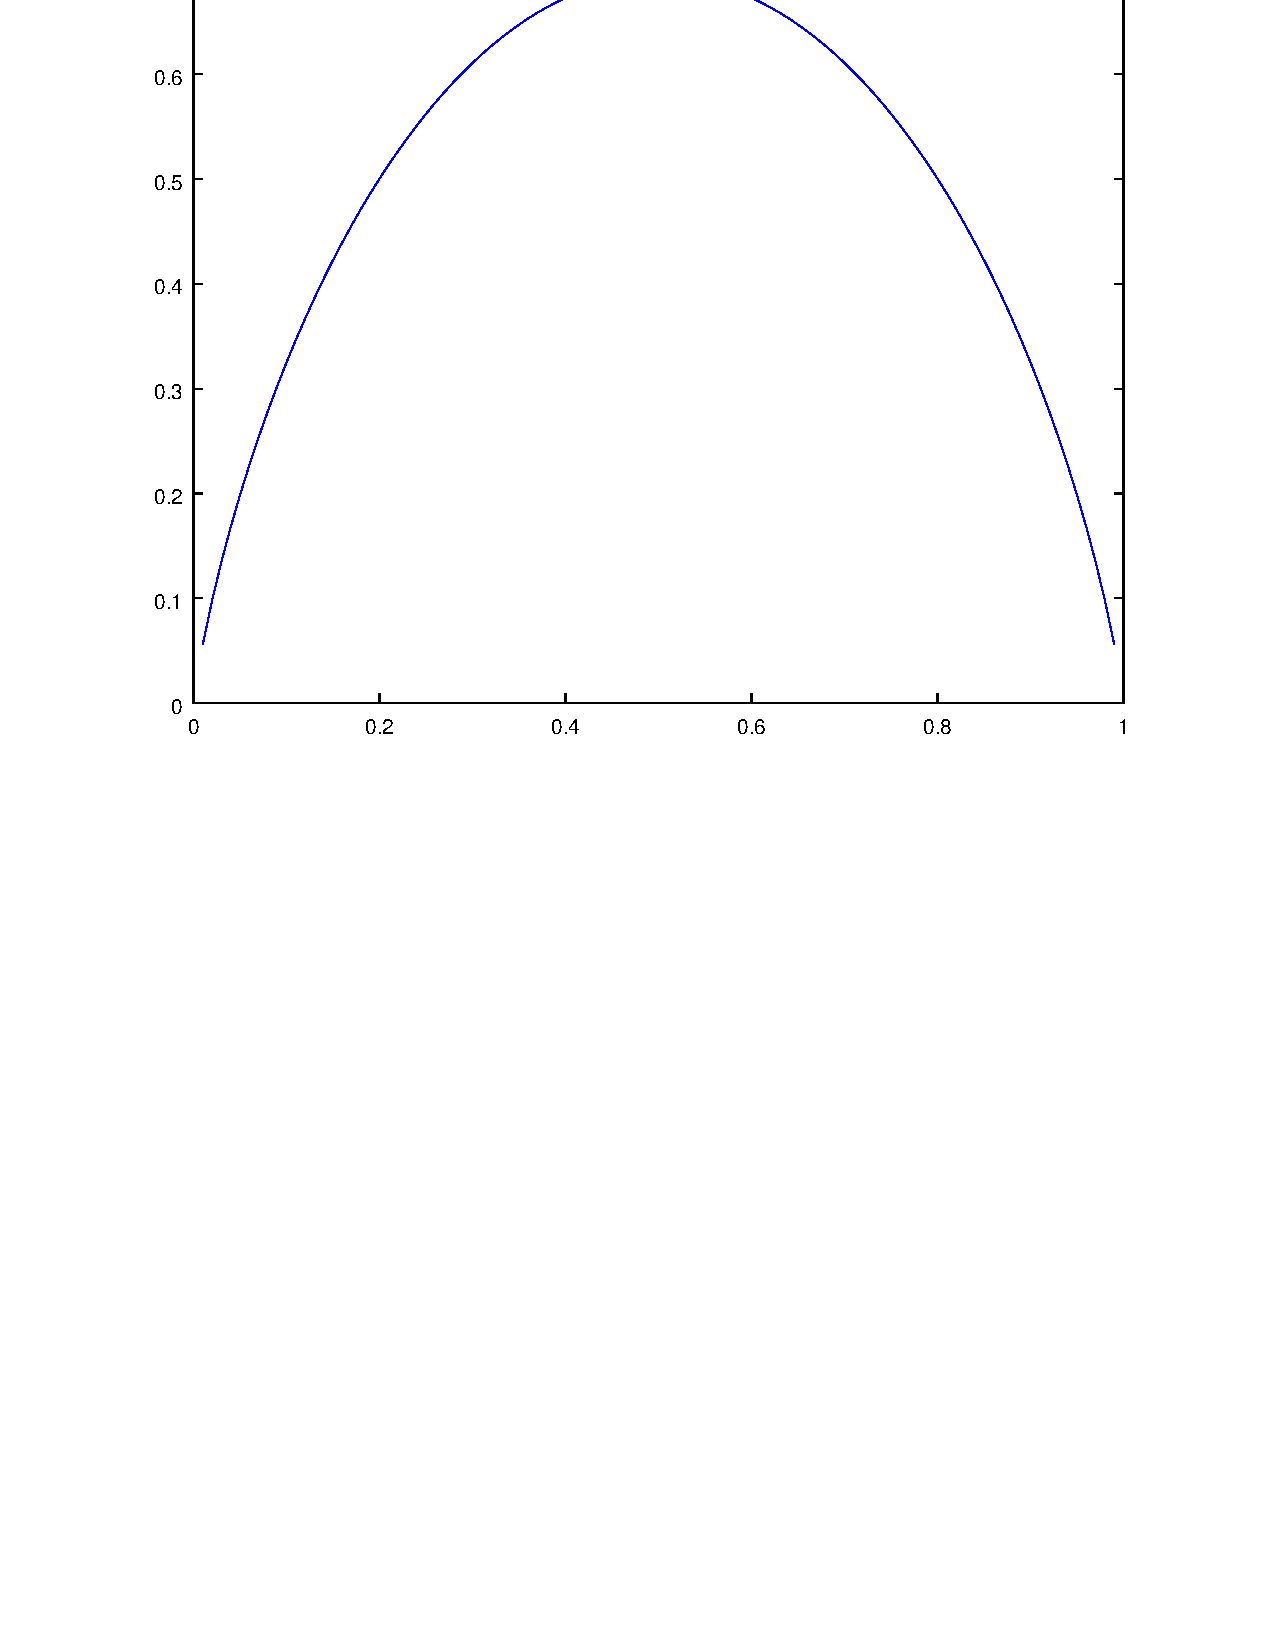
\includegraphics[width=\textwidth]{PlotA2c.pdf}
\end{figure}



\end{document}
